\begin{exercise}[ID=Q201001, difficulty=easy, type=ER, typequestion=open]
    Maria usou um livro de receitas para fazer um bolo de fubá. Mas, ao fazer a tradução do livro do inglês para o português, a temperatura permaneceu em Fahrenheit ($^\circ F$). A receita disse que o bolo deve ser levado ao forno a $392\;^\circ F$ e permanecer nessa temperatura por 30 minutos. Qual é a temperatura em graus Celsius que Maria deve deixar o forno para não errar a receita?
\end{exercise}
\begin{shortsolution}
	$200\;^\circ C$.
\end{shortsolution}
\begin{solution}
	Dado que $T_{F}=392\;^\circ F$ e utilizando a equação de conversão entre Celsius e Fahrenheit, temos: \[\dfrac{T_{C}}{5}=\dfrac{392-32}{9}\] Desta forma, isolando $T_{C}$, obtemos: \boxed{T_{C}=200\;^\circ C}
\end{solution}

\begin{exercise}[ID=Q201002, difficulty=easy, type=ER, typequestion=open]
    Determine o valor da temperatura de zero absoluto nas escalas Celsius e Fahrenheit.
\end{exercise}
\begin{shortsolution}
	$-273\;^\circ C$ e $-459,4\;^\circ F$.
\end{shortsolution}
\begin{solution}
	A temperatura de zero absoluto é igual a $0\;K$.\\Utilizando a equação de conversão entre Celsius e Kelvin, temos: \[T_{C}=0-273\] Logo, isolando $T_{C}$, obtemos: $T_{C}=-273\;^\circ C$.\\ Agora, utilizando a equação de conversão entre Fahrenheit e Kelvin, temos: \[\dfrac{T_{F}-32}{9}=\dfrac{0-273}{5}\] Logo, isolando $T_{F}$, temos: $T_{F}=-459,4\;^\circ F$.\\ Assim, podemos concluir que: \boxed{0K=-273\;^\circ C=-459,4\;^\circ F}    
\end{solution}

\begin{exercise}[ID=Q201003, difficulty=easy, type=ER, typequestion=open]
    Determine a única temperatura cuja indicação é a mesma nas escalas Celsius e Fahrenheit.
\end{exercise}
\begin{shortsolution}
$-40\;^\circ$
\end{shortsolution}
\begin{solution}
	A condição é $T_{C}=T_{F}=T$. Portanto, substituindo na equação de conversão entre Celsius e Fahrenheit, temos o seguinte: \[\dfrac{T}{5}=\dfrac{T-32}{9}\] Assim, isolando $T$, obtemos: \boxed{T=-40\;^\circ}\\
	Logo, $-40\;^\circ C$ é igual a $-40\;^\circ F$.    
\end{solution}

\begin{exercise}[ID=Q201004, difficulty=easy, type=ER, typequestion=open]
    O verão de 1994 foi particularmente quente nos Estados Unidos da América. A diferença entre a máxima temperatura do verão e a mínima no inverno anterior foi de $60\;^\circ C$. Qual o valor dessa diferença na escala Fahrenheit?
\end{exercise}
\begin{shortsolution}
	$108\;^\circ F$
\end{shortsolution}
\begin{solution}
	A relação entre a variação de temperatura na escala Fahrenheit e a escala Celsius é a seguinte: $\Delta 1\;^\circ C=\Delta 1,8\;^\circ F$.\\ Desta forma, a partir de uma proporção simples, obtemos: \[\dfrac{x}{1,8}=\dfrac{60}{1}\] Logo, \boxed{x=108\;^\circ F}\\ Ou seja, uma variação de $60\;^\circ C$ equivale a uma variação de $108\;^\circ F$.   
\end{solution}

\begin{exercise}[ID=Q201005, difficulty=easy, type=ER, typequestion=open]
    O cientista francês René Réaumur criou uma escala muito usada no passado, que adotava os seguintes valores: $0\;^\circ R$ para o ponto de gelo e $80\;^\circ R$ para o ponto vapor, ambos sob pressão normal. Calcule a temperatura nessa escala correspondente a $35\;^\circ C$.
\end{exercise}
\begin{shortsolution}
	$28\;^\circ R$
\end{shortsolution}
\begin{solution}
	Utilizando proporção entre as escalas, obtemos o seguinte: 
	\[\dfrac{35-0}{100-0}=\dfrac{T_{R}-0}{80-0}\]
	Assim, após isolarmos $T_{R}$, encontramos que: \boxed{T_{R}=28\;^\circ R}\\ Ou seja, $35\;^\circ C=28\;^\circ R$.    
\end{solution}

\begin{exercise}[ID=Q201006, difficulty=medium, type=ER, typequestion=open]
    Um estudante de física criou uma escala ($^\circ X$), comparada com a escala Celsius ele obteve o seguinte gráfico:
    \begin{figure}[ht] 
        \centering
        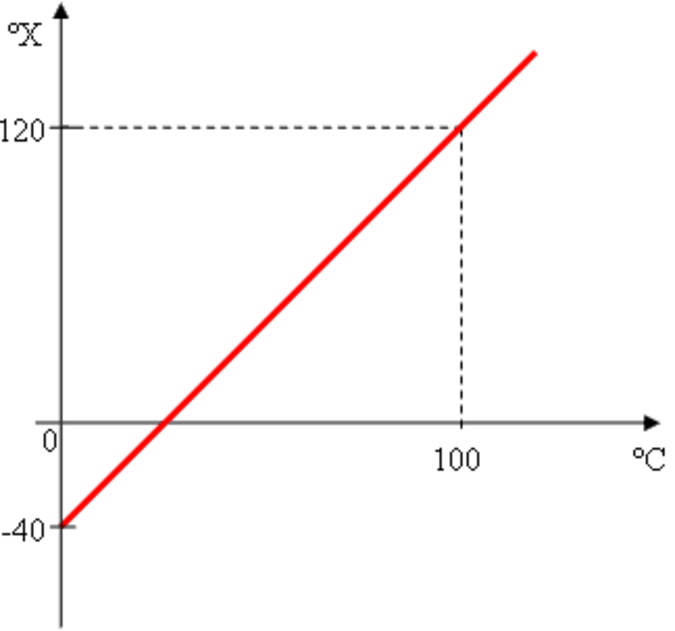
\includegraphics[scale=0.3]{graph1.pdf}
        %\caption{Exercício}
        \label{fig:graphterm1}
    \end{figure}
    \begin{enumerate}[label=\alph*),nosep]
        \item Qual a equação de conversão entre a escala $X$ e a escala Celsius?
        \item Qual a temperatura do corpo humano ($37\;^\circ C$) nesta escala?
    \end{enumerate}
\end{exercise}
\begin{shortsolution}
	$19,2\;^\circ X$
\end{shortsolution}
\begin{solution}
	\noindent
\begin{enumerate}[label=\alph*),nosep]
	\item A partir do gráfico, é possível escolher dois pontos $P_{1}=(-40,0)$ e $P_{2}=(100,120)$. Fazendo uma proporção entre as escalas, obtemos:
	\[\dfrac{T_{X}-(-40)}{120-(-40)} = \dfrac{T_{C}-0}{100-0}\]
	Desta forma:
	\[\boxed{T_{X}=\dfrac{8 \cdot T_{C}}{5} - 40}\]
	\item Substituindo $37\;^\circ C$ na relação anterior, encontramos: \boxed{19,2\;^\circ X}
\end{enumerate}   
\end{solution}